\documentclass[10pt]{beamer}
\usepackage[utf8]{inputenc}
\usepackage[T1]{fontenc}
\usepackage{lmodern}
\usetheme{Antibes}
%\mode<presentation>
%{
%	\usetheme{Darmstadt}      % or try Darmstadt, Madrid, Warsaw, ...
%	\usecolortheme{beaver} % or try albatross, beaver, crane, ...
	\usefonttheme{serif}  % or try serif, structurebold, ...
%	\setbeamertemplate{navigation symbols}{}
	\setbeamertemplate{caption}[numbered]
%} 
 \setbeamertemplate{navigation symbols}{} 

\setbeamertemplate{headline}[10mm]
\setbeamertemplate{footline}[page number]

\setbeamertemplate{blocks}[rounded][shadow=true]% 要将上述示例幻灯片中围绕定理的盒子改成圆角并添加阴影
\usepackage{ctex} %增加中文处理
\usepackage[english]{babel}
\title[画出的导线 Conducting Lines]{Conducting Lines\\画出的导线}
\author{Problem 10}
\institute[BIT]{Number: 1017}
\date{\today}


\linespread{1.1}
\begin{document}
	%\author{}
	%\title{}
	%\subtitle{}
	%\logo{}
	%\institute{}
	%\date{}
	%\subject{}
	%\setbeamercovered{transparent}
	%\setbeamertemplate{navigation symbols}{}
	\begin{frame}
		\titlepage
	\end{frame}
	
	
	% Uncomment these lines for an automatically generated outline.
	\begin{frame}{Outline}
		\tableofcontents
	\end{frame}
	
	
	\section[问题重述 Problem Restatement]{问题重述 Problem Restatement}
	\begin{frame}{问题重述 Problem Restatement}
		\begin{center}
			\textit{\Large A line drawn with a pencil on paper can be electrically conducting. Investgate the characteristics of the conducting line.}
			
			\bigskip
			{\large 用铅笔在纸上画的线可以导电,研究这种导电特性。}
		\end{center}
	\end{frame}
	
	
	\section{问题分析 Problem Analysis}
	\begin{frame}{问题提出 Problem Posing}
		\begin{center}
			{\LARGE  \textit{为什么铅笔画出的线会导电?}}\\
			\large Why a line drawn with
			a pencil can be electrically conducting?
			
		\end{center}
	\end{frame}
	
	\begin{frame}{铅笔芯的构成 Composition of Pencil Lead}
		
		\qquad     一般来说,铅笔的笔芯都是用\textbf{石墨和粘土}按一定比例\textbf{混合}制成的。如"H"即英文"Hard"(硬)的词头,代表粘土
		,用以表示铅笔芯的硬度。"H"前面的数字越大(如6H),铅笔
		芯就越硬,即笔芯中粘土比例越大,写出的字越不明显,常用来
		复写。"B"是英文"Black"(黑)的词头,代表石墨,用以表示铅
		笔芯质软的情况和写字的明显程度。"B"前面的数字越大(如14B)
		,铅笔芯中石墨比例越大,写出的字越明显,常用以绘画,普通铅
		笔标号则一般为"HB"。
	\end{frame}
	
	
	
	
	\begin{frame}{石墨导电的原理 How Graphite Conducts Electricity}
		\textbf{石墨是导电体}:\\
		\qquad 石墨是碳的同素异形体,而碳是四价
		原子。每个碳原子最外层有4个电子,与
		周围的碳原子形成六元环时共用3个电子,
		这样的话就会有一个\textbf{多余的自由电子},它在
		外加电场的作用下会发生定向移动,从而
		导电。
	\end{frame}
	
	\section[实验设置 Experimental Setup]{实验设置 Experimental Setup}
	\begin{frame}{实验器材 Experimental equipment}
		\begin{itemize}
			\item 万用表
			\item 2H HB 2B 4B 6B 8B 等铅笔
			\item 温度计
			\item 直尺
			\item 纸张等
		\end{itemize}
	\end{frame}
	
	
	\begin{frame}{实验方法 Experimental Methods}
		

			\textbf{实验核心方法:}
			\begin{itemize}
			\item 运用\textbf{控制变量法}分别分析所画的线在不同石墨含量、长度、宽度和温度下的电阻变化规律。\bigskip
			\end{itemize}
	
		\bigskip
	\textbf{误差控制方法:}
	\begin{itemize}
	\item 每条线都用铅笔画10次,以保证厚度相同。
	\item 测量多次取平均值。
\end{itemize}\bigskip

\textbf{温度控制方法:}
		\begin{itemize}
			\item 利用冰箱使温度达到-20°C,并测量电阻。
			\item 在常温下测量电阻。
			\item 利用吹风机加热后测量电阻。
		\end{itemize}
	\end{frame}
	
	
	\section{理论分析及实验结果 Theoretical Analysis and Experimental Results }
	\subsection{石墨含量 Graphite Content}
	
	
	\begin{frame}%{理论模型 Theoretical Model}
		\begin{itemize}
			\item {\LARGE \textit{石墨含量 Graphite Content}}
			\item 长度和宽度 Length and Width
			
			\item 温度 Temperature
			\item 接触电阻 Contact Resistance
		\end{itemize}
	\end{frame}
	
	
	\begin{frame}{常见铅笔中石墨与粘土的含量 \\The Ratio of Graphite and Clay}
		\begin{table}[htp]
			\caption{常见铅笔中石墨与粘土的含量}
			\centering
			\begin{tabular}{||c|c|c||}
				\hline
				铅笔类型&石墨占比(\%)&粘土占比(\%) \\ 
				\hline 
				2H&47  &53  \\ 
				\hline 
				HB&64  &36  \\ 
				\hline 
				2B&78  &22  \\ 
				\hline 
				3B&80  &20  \\ 
				\hline 
				4B&84  &16  \\ 
				\hline 
			\end{tabular} 
		\end{table}
		\pause
		
	\end{frame}
	
	\begin{frame}{实验结果 Experimental Result}
		利用2H至10B的不同铅笔画线(长15cm,宽2mm),并测量其电阻,得到如下结果:
		
	\end{frame}
	
	
	\begin{frame}{实验结果 Experimental Result}
		利用2H至10B的不同铅笔画线(长15cm,宽2mm),并测量其电阻,得到如下结果:
		
	\end{frame}
	
	
	\begin{frame}%{理论模型 Theoretical Model}
		\begin{itemize}
			
			\item 石墨含量 Graphite Content
			\item {\LARGE \textit{长度和宽度 Length and Width}}
			\item 温度 Temperature
			\item 接触电阻 Contact Resistance
		\end{itemize}
	\end{frame}
	
	
	\subsection{长度和宽度 Length and Width}
	\begin{frame}{石墨线模型}
		因纸张表面极为粗糙,如下所示:
	
		因而建立石墨线的模型如下:
		
		
	\end{frame}
	\begin{frame}{公式 Equations}
		\begin{theorem}
			$$R=\rho\frac{L}{S}$$ \\
			\begin{center}
				$ R $为电阻,$ \rho $为电阻率,$ L $为长度,$ S $为横截面积。
			\end{center}
		\end{theorem}
		\pause
		\begin{theorem}
			$$ S=W\cdot D $$
			\begin{center}
				$W$为Width 宽度,$ D $为Depth 深度。
			\end{center}
		\end{theorem}
	\end{frame}
	
	
	\begin{frame}{实验结果 Experimental Result}
		利用6B铅笔画出一长15cm宽2mm的石墨线,在不同接入长度下对其电阻进行测量,所得数据如下:
		
	\end{frame}
	
	
	\begin{frame}{实验结果 Experimental Result(Continue)}
		利用6B铅笔画出一长5cm宽度以5mm跳变的石墨线群,分别测量其电阻,并将结果展示为电阻和宽度的倒数$ \frac{1}{W} $的关系:
		
	\end{frame}
	
	
	%\begin{frame}{实验结果 Experimental Result(Continue)}
	%	利用6B铅笔画出一长5cm宽度以5mm跳变的石墨线群,分别测量其电阻,并将结果展示为电阻和宽度的$ {W} $的关系:
	%	\begin{figure}
	%		\centering
	%		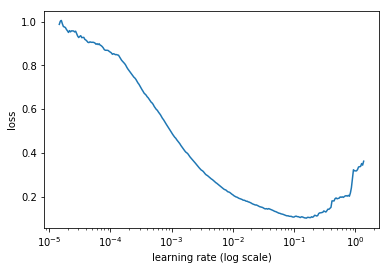
\includegraphics[width=0.8\linewidth]{figs/f8}
	%		\label{fig:f3}
	%	\end{figure}
	%\end{frame}
	
	
	\subsection{温度 Temperature}
	\begin{frame}%{理论模型 Theoretical Model}
		\begin{itemize}
			\item 石墨含量 Graphite Content
			\item 长度和宽度 Length and Width
			\item {\LARGE \textit{温度 Temperature}}
			\item 接触电阻 Contact Resistance
		\end{itemize}
	\end{frame}
	
	\begin{frame}{实验准备 The Preparation of Experiment}
		\textbf{\textit{研究对象:}}长5cm,宽5mm的6B铅笔画线。
		\bigskip
		
		\textbf{\textit{实验器材:}}红外温度计、冰箱(-20°C、1°C环境)、吹风机(49°C、59°C环境)\pause
		
	\end{frame}
	
	\begin{frame}{实验结果 Experimental Result}
		
		\begin{theorem}
			\[ R=\alpha T+0.3536(M\Omega), T(^\circ C) \]
			\[ R=\alpha T-0.3849(M\Omega), T(K) \]
			$$ \alpha\text{为温度系数,其值为}-0.0027M\Omega /K $$
			
		\end{theorem}
	\end{frame}
	
	\begin{frame}{温度的影响 The Influence of Temperature }
		
		\qquad 接入电压后画线电阻因热效应温度升高,从而阻值降低。由$ P=\frac{U^2}{R} $知,会产生更大的热量,从而温度升高,阻值降低。这是一个正反馈系统,但是这种状态不能长时间保持。
	\end{frame}
	
	\begin{frame}{对温度影响的分析 The Analysis of the Temperature-Influence}
		\qquad 画线电阻的阻值为$ M\Omega(10^6) $量级。假设电源电压为$ 10V\sim 100V $,那么根据公式$ P=\frac{U^2}{R} $,可以计算出画线电阻功率$ P $的数量级为$ 10^{-4}\sim 10^{-2} $,此功率对于温度的影响较小,在电源电压$ 100V $以下时可以忽略不计。
		
		\bigskip
		\pause
		{\large \textbf{结论:外接一般电源后,画线电阻阻值可以认为保持不变。}}
	\end{frame}
	\subsection{接触电阻 Contact Resistance}
	\begin{frame}%{理论模型 Theoretical Model}
		\begin{itemize}
			\item 石墨含量 Graphite Content
			\item 长度和宽度 Length and Width
			\item 温度 Temperature
			\item {\LARGE \textit{接触电阻 Contact Resistance}}
		\end{itemize}
	\end{frame}
	
	\begin{frame}{接触电阻分析 The Analysis of Contact Resistance }
		\textbf{	\textit{分析一:}}
		
		\qquad 画线长度$ L $与阻值$ R $成正相关。
		\begin{theorem}
			\begin{center}
				$R_{\text{总}}=\beta_1L+C_1$, 其中$ \beta_1=\frac{\rho}{W\cdot D} $
			\end{center}
		\end{theorem}
		\qquad $ R_{\text{总}} $由实际电阻$ R_{\text{实际}} $和接触电阻$ R_{\text{接触}} $组成,而$ R_{\text{实际}} $与长度$ L $成正比,即$ R_{\text{实际}} =\beta_1L$,则$ R_{\text{接触}} =C_1$,即截距大小。
		\pause
		
		\bigskip
		\textbf{	\textit{分析二:}}
		
		\qquad 宽度$ W $的倒数和阻值$ R $正相关。
		\begin{theorem}
			\begin{center}
				$R_{\text{总}}=\beta_2\cdot \frac{1}{W}+C_2$, 其中$ \beta_2=\frac{\rho L}{ D} $
			\end{center}
		\end{theorem}
		\qquad $ R_{\text{总}} $由实际电阻$ R_{\text{实际}} $和接触电阻$ R_{\text{接触}} $组成,而$ R_{\text{实际}} $与宽度的倒数$ \frac{1}{W} $成正比,即$ R_{\text{实际}} =\beta_2\cdot \frac{1}{W}$,则$ R_{\text{接触}} =C_2$,即截距大小。
	\end{frame}
	

	
	\section[Conclusion]{结论 Conclusion}
	\begin{frame}{铅笔画线的总结 Conclusion}
		\begin{enumerate}
		 {\large \item 画线\textbf{长度}与阻值成\textbf{正}相关
			\item 画线\textbf{宽度}与阻值成\textbf{负}相关
			\item \textbf{石墨含量}与阻值成\textbf{负}相关
			\item 画线\textbf{温度}与阻值成\textbf{负}相关}
		\end{enumerate}
	\end{frame}
	
	\section[Reference]{参考文献 Reference}
	
	\begin{frame}{参考文献 Reference}
		[1] https://www.zhihu.com/question/51313311/answer/860906178
		
		[2] S.Rattanaweeranon, et al. Influence of Bulk Graphite Density on Electricity Conductivity[J]. Porcedia Engineering, 2012(32): 1100-1106.
		
		[3] https://www.bilibili.com/video/av65447558
		
		[4] ANDRE K. GEIM, PHILIP KIM. CARBON WONDERLAND[J]. Scientific American, 2008, 4(4): 68-75.
		
		[5] 张昊东, 陈靖雯, 张灵聪, 陈京. 基于还原氧化石墨烯的疏水亲油膜的制备及其在油水分离中的应用[J]. 化工新型材料, 2019, 47(06): 223-227.
		
		[6] https://www.zhihu.com/question/51313311/answer/860906178
		
		[7] 张福勤, 黄启忠, 黄伯云, 巩前明, 陈腾飞. C/C复合材料石墨化度与导电性能的关系[J]. 新型炭材料, 2001(02): 45-48.
	\end{frame}
	
	\begin{frame}
		\begin{center}
			\Huge \textit{谢谢聆听!}
		\end{center}
		
	\end{frame}
\end{document}